\newcommand{\proxytotalphishing}{6,350\xspace}
\newcommand{\proxyevadephishing}{6,136\xspace}
\newcommand{\proxyphishingperc}{96.62\%\xspace}


\section{Evaluation}
\label{s:eval}

We implement \spartacus as a Chrome browser extension, which the anti-phishing ecosystem can leverage and spread trivially.
We deploy the prototype locally in three machines.
We did not conduct user study for \spartacus because we simulate the user's environment from our side.
and evaluate it from three perspectives, including effectiveness, latency, and potential impact on benign websites.
These three aspects demonstrate the feasibility of the \spartacus framework in practice because it can successfully evade advanced phishing websites, can negligibly introduce latency to the users when visiting websites, and can run in the backstage without causing errors on benign websites.

\noindent
\textbf{Dataset.}
In our evaluation, we use two different datasets, a malicious one, to test the effectiveness of \spartacus, and a benign one, for the understanding of its potential impact on benign websites.

\noindent
(1)~\emph{APWG Dataset}:
For the effectiveness evaluation, \spartacus visits 160,728 live phishing websites from November 2020 to July 2021 using Anti-Phishing Working Group (APWG) URL feed~\cite{ecrimeexchange},
which is a curated dataset for reported phishing URLs, supported by a large number of collaborated members.
Additionally, we leverage another~\proxytotalphishing live phishing websites in the APWG Dataset to evaluate the effectiveness of IP mutation.

\noindent
(2)~\emph{Benign Dataset}:
To evaluate the potential impact on benign websites, \spartacus leverages a dataset of 60,848 benign domains, which is randomly selected from 629,843 domains in Alexa Top One Million Domain List~\cite{AlexaTop1M}.

% \subsection{Support From the Ecosystem}

% \spartacus focuses on the evasion of advanced phishing attacks,
% because the current anti-phishing techniques can effectively and efficiently detect and blacklist basic phishing~\cite{oest2020phishtime}.

% We still need to measure the ability of current anti-phishing systems against basic attacks.
% To this end, we submit phishing URLs to one of the systems, Google Safe Browsing (GSB), the same time when \spartacus inspects them.
% Meanwhile, we keep querying GSB for the blacklist result to calculate the blacklist speed.



\subsection{Effectiveness}
\label{ss:effectiveness}

\begin{figure*}
\centering
	\begin{subfigure}[tb]{.31\textwidth}
		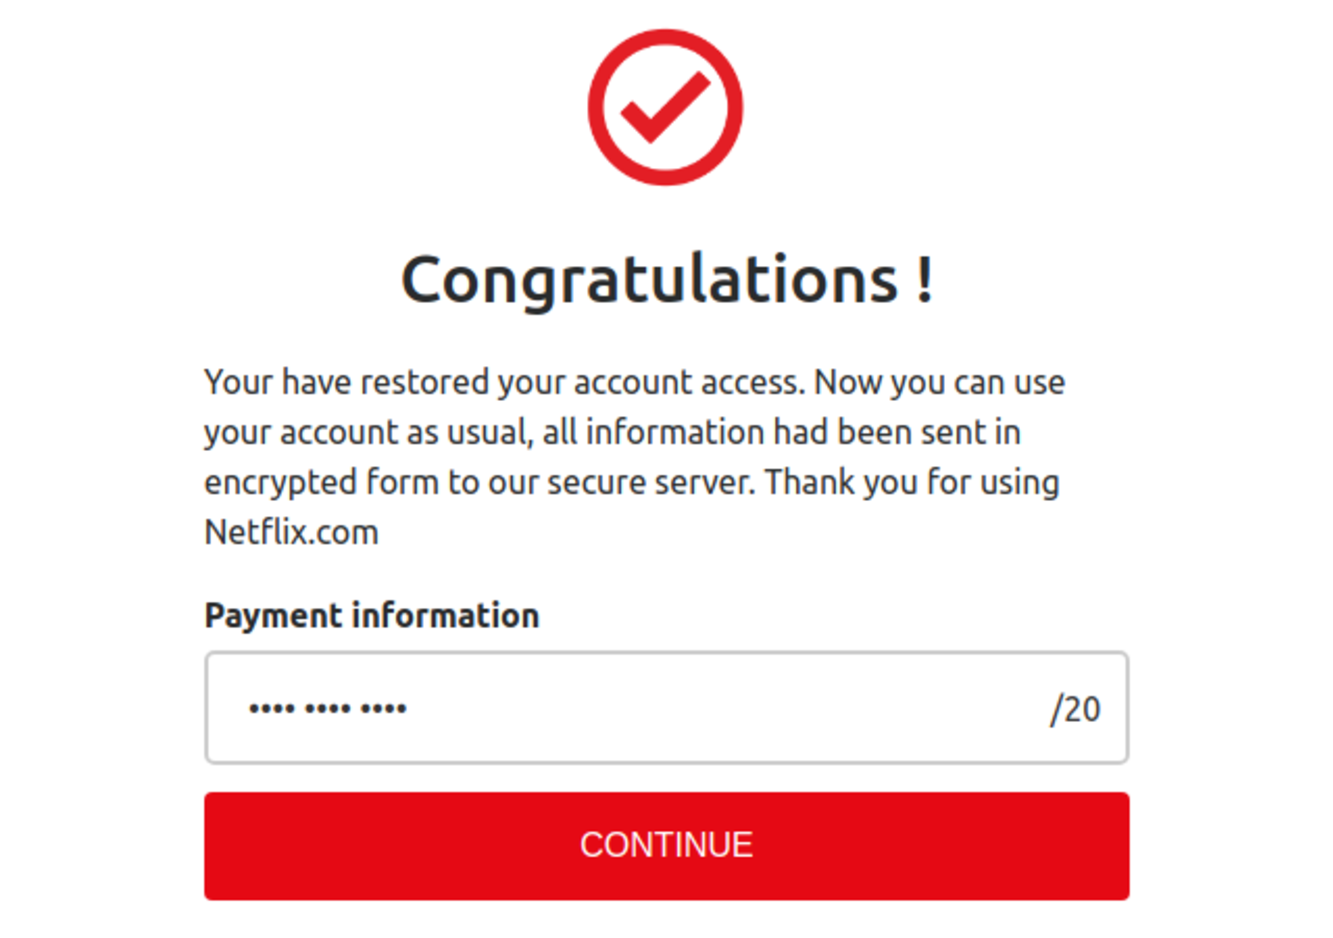
\includegraphics[width=\linewidth]{figs/netflix_n.pdf}
        \caption{Default browser visit.}
        \label{fig:normal}
	\end{subfigure}%
	\quad
	\begin{subfigure}[tb]{.31\textwidth}
		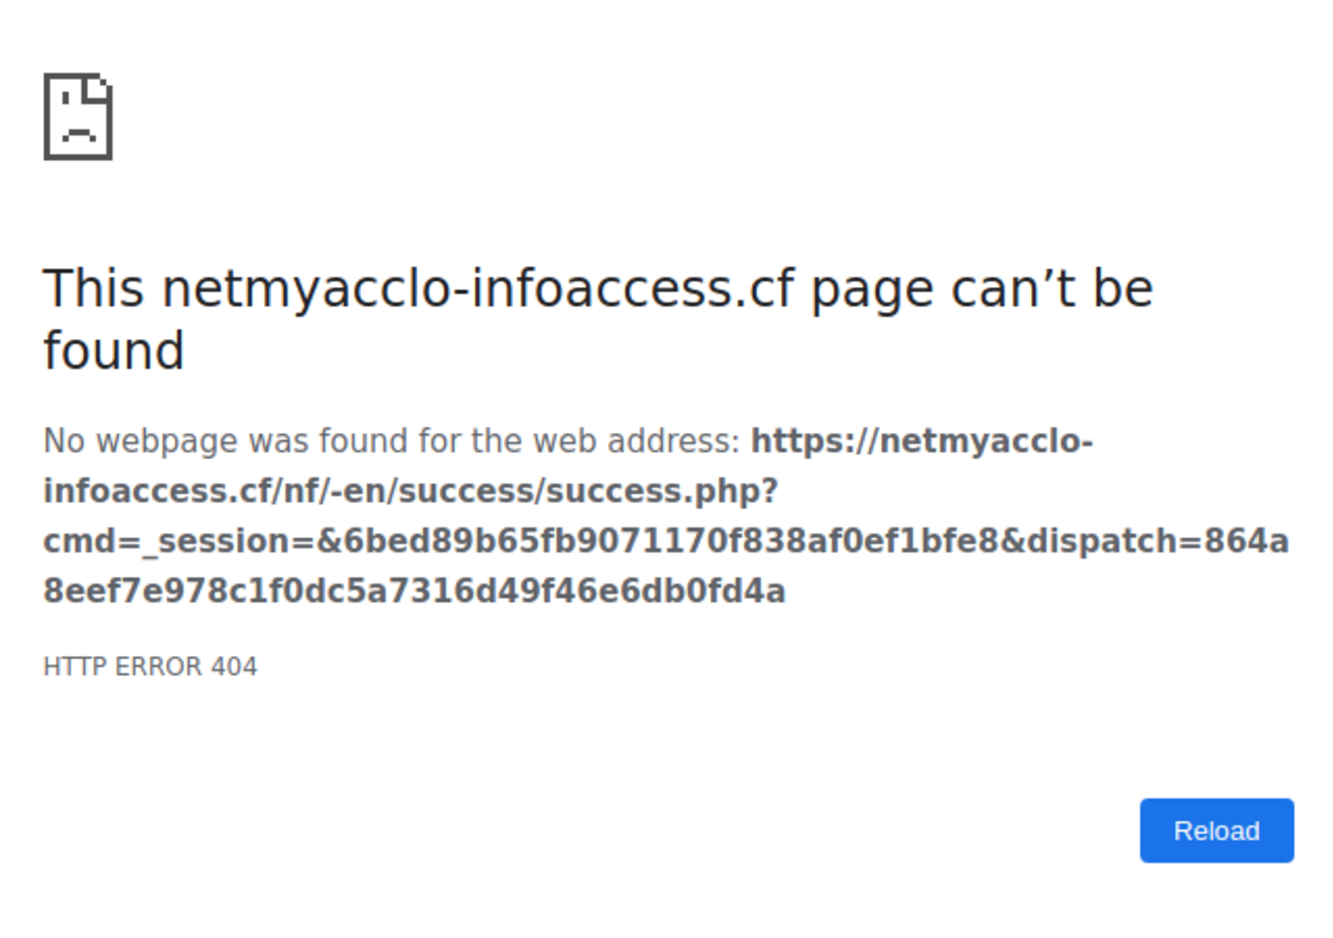
\includegraphics[width=\linewidth]{figs/netflix_sp.pdf}
        \caption{\spartacus browser visit with error.}
        \label{fig:sp1}
	\end{subfigure}%
	\quad
	\begin{subfigure}[tb]{.31\textwidth}
		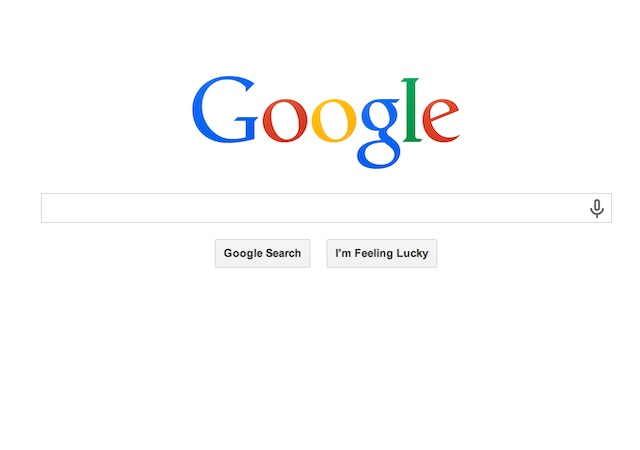
\includegraphics[width=\linewidth]{figs/netflix_sp2.png}
        \caption{\spartacus browser visit with content.}
        \label{fig:sp2}
	\end{subfigure}%
	\quad
% 	\vspace{-5pt}
	\caption{Web page contents from default and \spartacus'ed browser visits for a cloaked phishing website.}
	\label{fig:effectiveness}
% 	\vspace{-10pt}
\end{figure*}

We evaluate the effectiveness of \spartacus automatically by conducting an experiment where we visit same phishing websites with different configurations of browsers, one with default user setting, the other with \spartacus to mutate the profile.
We simulate the default setting browser as normal users and the one with \spartacus as users with our framework.
The phishing URLs both browsers visit are from the APWG Dataset.
For each visit, we record the final landing web page content and URL.
Either a legitimate final URL or a non-malicious web page content indicates the success of \spartacus evading phishing content for users.
If there is still malicious content shown to \spartacus, it indicates that either the phishing website does not contain advanced evasion techniques, or \spartacus does not trigger them with current fingerprint.
For the first situation, the current anti-phishing ecosystem has proposed methodologies to mitigate basic phishing attacks with effectiveness and efficiency.
As for the second, we believe that by visiting the same website with different configurations of HTTP requests mutated by \spartacus, the evasion techniques embedded in the phishing website can be triggered eventually. 

We examined 160,728 phishing URLs from APWG from November 2020 to July 2021,
132,247 (82.28\%) of which do not contain malicious content, just by mutating User-Agent and Referrer in \spartacus.
We consider an HTTP response benign if (1) its web page content does not contain maliciousness, such as phishy words or bad forms, according to the content features stated in CANTINA+~\cite{xiang2011cantina+};
% (2) the response status code is an error one (4XX/5XX);
or (2) the destination domain is legitimate, excluding web hosting service domains.
\autoref{fig:effectiveness} demonstrates the difference of response web page content between default and \spartacus'ed browser visit for a cloaked phishing websites.
The content in~\autoref{fig:normal} shows the phishing content when a real person visits it.
On the other hand, 
% when \spartacus appends a bot-looking string to the existing User-Agent, such as~\emph{bot},
when \spartacus mutates the HTTP profile,
the phishing server considers the visit as from an anti-phishing infrastructure.
Thus, it denies the request from \spartacus and an error web page is shown as~\autoref{fig:sp1}.
On the other hand, advanced phishing servers can redirect visit to a benign domain with status code of 200 instead of returning an error page.
In this way, \spartacus'ed browser will receive web page contents such as~\autoref{fig:sp2},
which also indicates a successful evasion.

The evaluation result shows that \spartacus can impersonate users as anti-phishing crawler and trigger the cloaking techniques of advanced phishing websites.
Because the web page content returned through \spartacus's visit does not contain any maliciousness, Internet users will not be trapped in the attack.


% \textcolor{blue}{eval result}

\subsection{Effectiveness of Triggering Words}

According to the design, the profile mutator of \spartacus selects one of 407 triggering words, following the order of their popularity in examined phishing kits.
So in this section, we evaluate the effectiveness of each triggering word on triggering fingerprinting cloaking techniques in phishing websites.

\newcommand{\senstotalphishing}{916\xspace}
\newcommand{\sensevadephishing}{725\xspace}

We test all the triggering words by appending each after the User-Agent string within \spartacus and then visiting the same phishing website.
Similarity to the evaluation of effectiveness of \spartacus, we also visit the website using a default browser as a comparison.
We conduct the experiment on \senstotalphishing phishing websites.
% Except \sensevadephishing websites that show same content on all HTTP profiles,
\sensevadephishing show web page differently at least under one triggering word between \spartacus'ed browser and default browser.

\evalsenswords

In \sensevadephishing cloaked phishing websites, the triggering words have different evasion abilities.
\autoref{tab:evalsenswords} is the result of top 10 effective triggering words evading phishing content in \spartacus.
In the table, word \emph{bot} has the most evasion record.
99.31\% of the cloaked phishing websites can be evaded by appending \emph{bot} in the User-Agent using \spartacus.
Compared with the rank in~\autoref{tab:topsenswords}, it is ranked first blocked word appearance in examined phishing kits.
The high effectiveness of this word confirms its high rank in the top used blocked words in the phishing kits.
Similarly, top effective words such as ``amazonaws'', ``phishtank'', and ``google'' also have a high usage in phishing kits.
On the other hand, word ``bot'' and ``amazonaws'' combined can make all tested cloaked phishing websites return benign content to users.

The evaluation result shows that our triggering word list can effectively evade phishing websites with fingerprinting cloaking techniques.
Furthermore, it indicates that a small number of triggering words can evade a myriad of cloaked phishing websites.


\subsection{Effectiveness of Proxy Server}

Even though \spartacus can successfully evade phishing content in over 80\% of the phishing websites by mutating User-Agent and Referrer string, 
it is still very important to update its arsenal so that \spartacus can use different weapons against different cloaking techniques (e.g., those who only check IP). 
Therefore, we conduct another experiment where \spartacus leverages a proxy server residing in Amazon AWS, where crawlers are often from, to visit phishing websites.
This experiment is to show the effectiveness of a crawler-like IP on evading cloaked phishing websites.


\spartacus visits \proxytotalphishing phishing websites by rerouting the request through the proxy server.
Similar to the evaluation procedure in~\Cref{ss:effectiveness},
we visit those websites in both default browser and \spartacus browser.
Then we compare the screenshot and HTML similarity of each phishing website on both sides.
Among the visited phishing websites, \proxyphishingperc (\proxyevadephishing) of them can be evaded by \spartacus through proxy server.
Therefore, \spartacus can evade phishing websites that implement IP, User-Agent, or Referrer cloaking.
Phishers may design emerging cloaking techniques in the future, but we design \spartacus as an extendable framework.
Additional fingerprints can be added into the existing framework to make it more evasive against cloaked phishing websites.


\subsection{Efficiency and Latency}

We need to make sure that \spartacus will not impact negatively on the user experience when they visit benign websites.
From the design of \spartacus, it will introduce latencies, including database query, HTTP profile mutation, and returned content inspection.
However, the latencies \spartacus introduces can be negligible.
Therefore, we conduct an experiment to measure the latency for the \spartacus system for the following three perspective, database query, profile mutation, and content inspection.
We leverage \emph{exthouse}~\cite{exthouse}, which analyzes the impact of a browser extension on web performance, as our test bench.
% We run exthouse with 1,000 phishing websites and 1,000 benign websites on two configurations of browsers, one with \spartacus, the other without, and compare the mean rendering time for each group of websites.
It contains five major measurements:
(1) Time to Interactive (TTI): the time it takes for the page to become fully interactive with the extension; 
(2) First Input Delay (FID $\Delta$): the time from when a user first interacts with the website to the time when the browser is actually able to begin processing event handlers in response to that interaction;
(3) Scripting Time (Scripting $\Delta$): the amount of time JavaScript execution in the extension;
(4) Long Task (Added Long Task): this value represents a sum of Long Tasks added by extension;
and (5) Extra CPU Consumption (Extra CPU Time): additional files in the extension need extra CPU consumption for each URL the browser visits.
The lower these three factors are, the better the website performs with the tested extension.
At last, \emph{exthouse} will score of the extension.
A higher score reflects a better performance of the extension.

\exthouse

\autoref{tab:exthouse} illustrates the metrics of top 10 Chrome extensions~\cite{exthouse} along with \spartacus when visiting benign and malicious websites under the inspection of \emph{exthouse}.
We test these extensions with 100 websites, including half benign and half malicious, and take the average into the metrics.
\spartacus has a score of 100, 20 ms FID, 0 scripting delta, and 800 ms of TTI when visiting benign websites.
The metrics of \spartacus visiting malicious websites also outscores those of other popular extensions.
Even though it takes long time to interact with the malicious website, it is still acceptable because \spartacus needs time to mutate the profile, which is still less than the time used consumed by other extensions.
Take \texttt{Avira Browser Safety} (ABS) as an example, it is an extension warning users if the website is unsafe.
However, it added long tasks and extra CPU time when visiting malicious websites.
As a similar type, \spartacus does not harden the CPU as ABS does.
At the same time, \spartacus can provide safe browsing for users.
The evaluation result means that with \spartacus, users can still interact with the website with minimum latency.
The inspection result shows that \spartacus out-scores popular Chrome extensions and does not impact the performance of websites, compared with other extensions.

\subsection{Impact on Benign Website}

Besides evading malicious content in phishing websites, \spartacus is also required to minimize the negative impacts on benign URL visit.
They can include ability of access the website, correct display of website layout, and correct functionalities of the website.
To evaluate the potential impacts to benign website, we conduct two experiments: Coarse-Grained and Fine-Grained.

\subsubsection{Coarse-Grained Experiment}

\coarsegrain

In Coarse-Grained experiment, we intend to evaluate if \spartacus system has negative impact on the access to the website or the website layout.
So we visit 60,848 (9.66\%) out of 629,843 URLs in Alexa Top One Million Domain List~\cite{AlexaTop1M} in both default and \spartacus'ed browsers.
We compare the web page screenshot and HTML similarity on the visited URLs.
The result is shown in~\autoref{tab:coarsegrain}.
After adopting~\Cref{alg:mutatelogic},
0.06\% (39) have different layouts and 
0.04\% (29) block the access from \spartacus'ed browser.

\begin{figure}[t]
    \centering
    \begin{subfigure}{0.48\linewidth}
        \centering
            
\includegraphics[width=\textwidth]{figs/38_normal.png}%
        \caption{Default browser visit.}
        \label{fig:coarse_normal}
    \end{subfigure}
    ~
    \begin{subfigure}{0.48\linewidth}
        \centering
            
\includegraphics[width=\textwidth]{figs/38_sp.png}
        \caption{\spartacus visit}
        \label{fig:coarse_sp}
    \end{subfigure}
    
    \caption{Difference due to the shape of buttons.}
    \label{fig:coarse}
    % \vspace{-10pt}
\end{figure}

\begin{figure}[t]
    \centering
    \begin{subfigure}{0.48\linewidth}
        \centering
            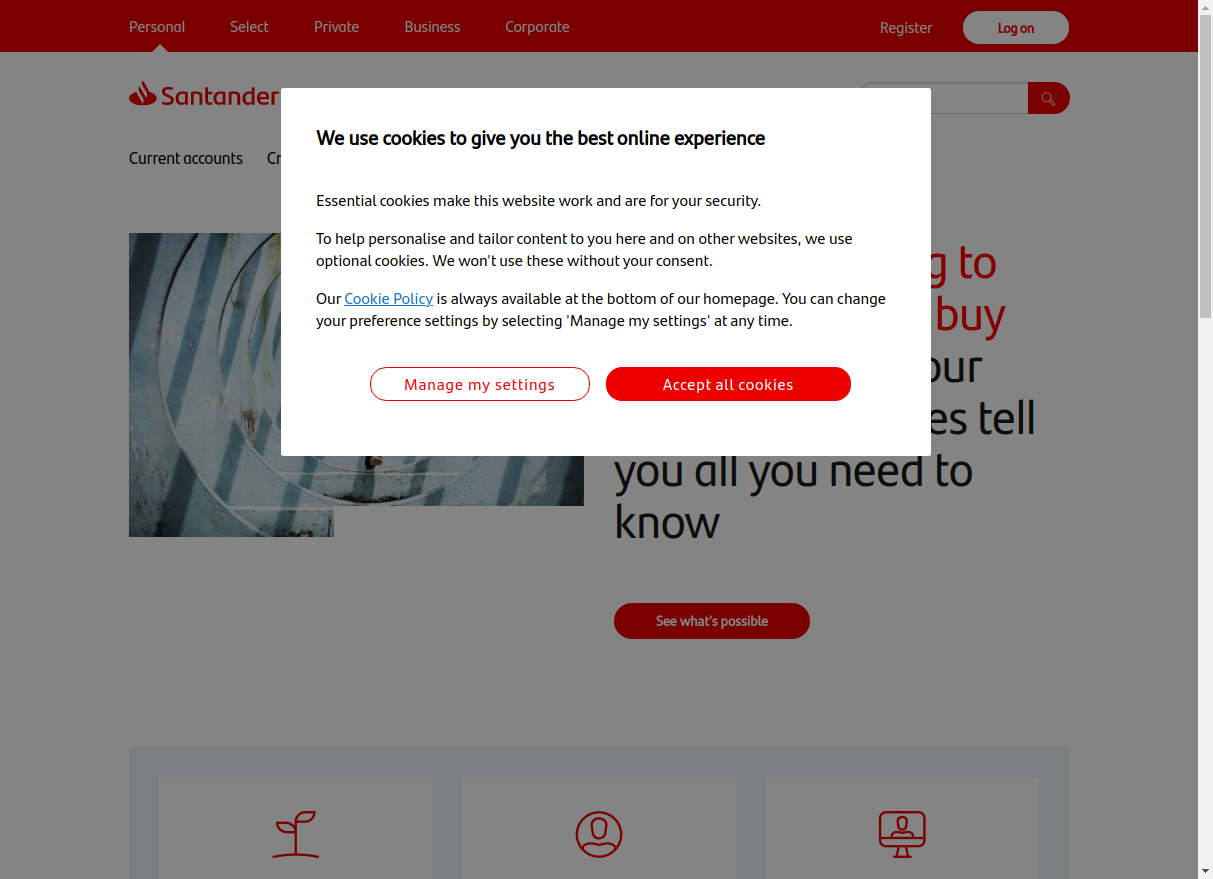
\includegraphics[width=\textwidth]{figs/2306_normal.png}%
        \caption{Default browser visit.}
        \label{fig:2306_normal}
    \end{subfigure}
    ~
    \begin{subfigure}{0.48\linewidth}
        \centering
            
\includegraphics[width=\textwidth]{figs/2306_sp.png}
        \caption{\spartacus visit}
        \label{fig:2306_sp}
    \end{subfigure}
    
    \caption{Difference due to popup.}
    \label{fig:2306}
    % \vspace{-10pt}
\end{figure}

We first examine the reason why \spartacus'ed browser show different layouts from the default browser.
And we find that although the screenshot and HTML similarity is not high between default and \spartacus browser visits,
to people, such difference does not impact them using or browsing the website.
For example, two web pages are different in terms of screenshot similarity between default and \spartacus browser visits shown in~\autoref{fig:coarse}.
The difference is due to the shape of buttons and different of background color.
% The change is on the scrolling promotion ads in the \texttt{div} tag.
% When the screenshot was captured in default visit, Ad One happened to show;
% and another Ad was in the way when \spartacus took the screenshot.
Similarly, in~\autoref{fig:2306}, a window popped up to ask for the permission of cookie in default browser, but did not in \spartacus's visit.
The cookie request pop-up missing in \spartacus browser is not due to the extension itself.
We visit the same website 10 times in different browsers without \spartacus, only for three times the pop-up appeared.
Even though our evaluation script can distinguish the difference between visits from two browsers,
users will not perceive that.
They can normally interact with the websites with \spartacus providing phishing-evading services.
% , which indicates that \spartacus does not make users perceive the difference, even if it has 




With applying~\Cref{alg:mutatelogic}, we evaluated \spartacus based on the threshold and find that 29 legitimate domains show different web page content on default and \spartacus'ed browsers, as listed in~\autoref{tab:coarsegrain}.
Hence, only 0.04\% of 60,848 domains are falsely evaded.
It is because the 29 domains do not meet the trustworthiness requirements and hence are not trusted by \spartacus.
% do not fall into the high reputation group of \spartacus's non-mutation criteria.
As one possible mitigation, we provide a channel for users to report falsely evaded websites.
Once receiving the report, we will conduct manual inspection and trust the false-positives.
% Additionally, 39 of the domains show different layouts between default and \spartacus browsers.
% As we discussed above, such difference will not affect the activities of normal users,
% but after applying~\Cref{alg:mutatelogic}, \spartacus and normal browsers perform more alike on benign domains.
As comparison, phishing URLs can still be evaded through \spartacus because they all triggered the condition to invoke \emph{mutate\_http\_profile()}.

\subsubsection{Fine-Grained Experiment}

\finegrain


In Fine-Grained experiment, we aim to exercise and evaluate the operation of websites visited through \spartacus.
It was inspired by the methodology used by Snyder et al.~\cite{snyder2017most} and Trickel et al.~\cite{trickel2019everyone}.
This methodology concentrates on the operation of a website from the perspective of the user.
Even though \spartacus may introduce an error to a website, the users do not perceive any difference when browsing, then we consider that \spartacus does not impact negatively on the website.
% evaluate potential impact \spartacus brings on the functionalities of benign domains.
This method of evaluation focuses more on potential impact \spartacus brings on the functionalities of benign domains than how \spartacus works.
And it was performed by the authors manually.

The experiment includes the evaluation of visibility of websites and interactions between visitor and the website.
It brings an additional metric that evaluates how \spartacus will influence users' daily activities.
There are four steps in the experiment.
(1) We open legitimate domains in a browser with \spartacus installed and also in one with default settings.
(2) We inspect the accessibility of the website, similar to the Coarse-Grained experiment.
(3) After the success of web page content retrieval, we compare the layouts between different visit.
(4) We interact with links, buttons, and other activities such as register/login, online chat, or shopping to make sure that the functionalities in a website perform correctly.
(5) At last, we test the authentication functionality to make sure that \spartacus extension will not impact it.

We randomly selected 60 domains from Alexa Top One Million List, especially 20 every 200 thousands.
The result is displayed in~\autoref{tab:finegrain}.
As a comparison, default browser has the same result as that of \spartacus.
Among the 60 legitimate domains, we can access 58 of them.
Two domains are inaccessible even in the default browser, so we suspect them offline already.
For the accessible 58 domains,
we follow the steps mentioned above to inspect them.
All of them have the same layout as the visit from the default browser.
Then we interact the 58 websites by clicking the buttons, chatting online, and adding items into the cart if it is a shopping website.
All 58 websites performed well.
At last, we register an account on 15 websites and they all allow us to do so.
Even though we can successfully register an account, we still need to make sure that we can log in properly with those accounts to test the authentication process under \spartacus.
The result shows that all the accounts we registered during the Fine-Grained experiment can be logged in successfully.
It means that the \spartacus system does not impact the authentication process in the website.

In summary, with the results retrieved from both coarse- and fine-grained experiment, we can summarize that \spartacus does not impact the accessibility and visibility on high reputation or long age domains, or its top reviewed subdomains.
Besides, for domains who can be accessed and displayed properly, the functionalities including links, buttons, and registration and authentication in the websites will not be affected.
Therefore, \spartacus can protect users from visiting advanced phishing websites while keep their normal browsing activities.

% \noindent
% \textbf{Database Query}.
% According to the e

% \noindent
% \textbf{Profile Mutation}.

% \noindent
% \textbf{Content Inspection}.

% \subsection{Privacy}

